\documentclass[tikz,border=5pt]{standalone}
\usepackage{amsmath,amssymb}
\usetikzlibrary{decorations.pathreplacing}
\begin{document}
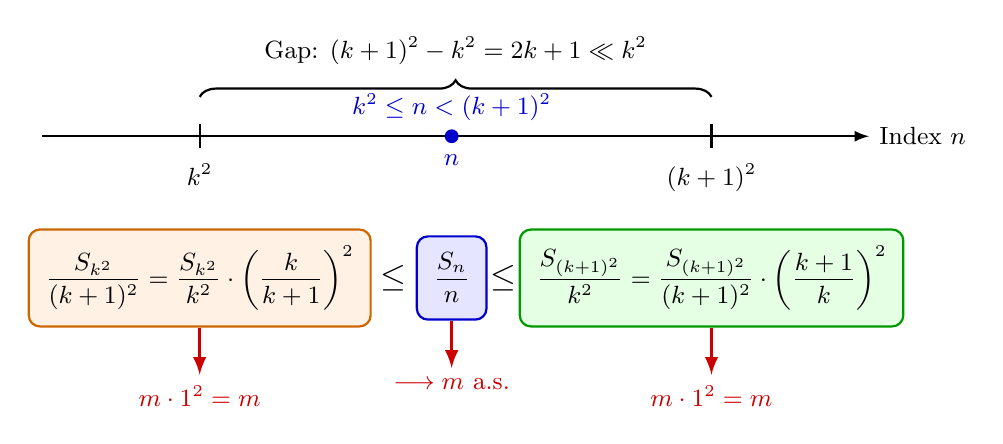
\begin{tikzpicture}[>=latex, font=\small]
  % Index axis
  \draw[->, thick] (0, 0) -- (10.5, 0) node[right] {Index $n$};

  \draw[thick] (2.0, 0.15) -- (2.0, -0.15) node[below=2pt] {$k^2$};
  \draw[thick] (8.5, 0.15) -- (8.5, -0.15) node[below=2pt] {$(k+1)^2$};

  \fill[blue!80!black] (5.2, 0) circle (2.5pt) node[below=3pt] {$n$};
  \node[above=2pt, blue!80!black] at (5.2, 0) {$k^2 \le n < (k+1)^2$};

  % Range bracket
  \draw[thick, decorate, decoration={brace, amplitude=6pt}] (2.0, 0.5) -- (8.5, 0.5)
    node[midway, above=8pt] {Gap: $(k+1)^2 - k^2 = 2k + 1 \ll k^2$};

  % Sandwiching inequalities
  \node[draw=orange!80!black, fill=orange!10, rounded corners, thick, inner sep=6pt] at (2.0, -1.8) (lower) {
    $\displaystyle \frac{S_{k^2}}{(k+1)^2} = \frac{S_{k^2}}{k^2} \cdot \left(\frac{k}{k+1}\right)^2$
  };

  \node[draw=blue!80!black, fill=blue!10, rounded corners, thick, inner sep=6pt] at (5.2, -1.8) (mid) {
    $\displaystyle \frac{S_n}{n}$
  };

  \node[draw=green!60!black, fill=green!10, rounded corners, thick, inner sep=6pt] at (8.5, -1.8) (upper) {
    $\displaystyle \frac{S_{(k+1)^2}}{k^2} = \frac{S_{(k+1)^2}}{(k+1)^2} \cdot \left(\frac{k+1}{k}\right)^2$
  };

  \path (lower) -- node[midway, font=\large] {$\le$} (mid);
  \path (mid) -- node[midway, font=\large] {$\le$} (upper);

  % Convergence arrows
  \draw[->, very thick, red!80!black] (lower.south) -- ++(0, -0.6) node[below] {$m \cdot 1^2 = m$};
  \draw[->, very thick, red!80!black] (mid.south) -- ++(0, -0.6) node[below] {$\longrightarrow m$ a.s.};
  \draw[->, very thick, red!80!black] (upper.south) -- ++(0, -0.6) node[below] {$m \cdot 1^2 = m$};
\end{tikzpicture}
\end{document}
